%%%%%%%%%%%%%%%%%%%%%%%%%%%%%%%%%%%%%%%%%%%%%%%%%%%%%%%%%%%%%%%%%%%%%
%% This is a (brief) model paper using the achemso class
%% The document class accepts keyval options, which should include
%% the target journal and optionally the manuscript type. 
%%%%%%%%%%%%%%%%%%%%%%%%%%%%%%%%%%%%%%%%%%%%%%%%%%%%%%%%%%%%%%%%%%%%%
\documentclass[journal=ENFL,manuscript=article]{achemso}

%%%%%%%%%%%%%%%%%%%%%%%%%%%%%%%%%%%%%%%%%%%%%%%%%%%%%%%%%%%%%%%%%%%%%
%% Place any additional packages needed here.  Only include packages
%% which are essential, to avoid problems later. Do NOT use any
%% packages which require e-TeX (for example etoolbox): the e-TeX
%% extensions are not currently available on the ACS conversion
%% servers.
%%%%%%%%%%%%%%%%%%%%%%%%%%%%%%%%%%%%%%%%%%%%%%%%%%%%%%%%%%%%%%%%%%%%%
\usepackage[version=3]{mhchem} % Formula subscripts using \ce{}

%%%%%%%%%%%%%%%%%%%%%%%%%%%%%%%%%%%%%%%%%%%%%%%%%%%%%%%%%%%%%%%%%%%%%
%% If issues arise when submitting your manuscript, you may want to
%% un-comment the next line.  This provides information on the
%% version of every file you have used.
%%%%%%%%%%%%%%%%%%%%%%%%%%%%%%%%%%%%%%%%%%%%%%%%%%%%%%%%%%%%%%%%%%%%%
%%\listfiles

%%%%%%%%%%%%%%%%%%%%%%%%%%%%%%%%%%%%%%%%%%%%%%%%%%%%%%%%%%%%%%%%%%%%%
%% Place any additional macros here.  Please use \newcommand* where
%% possible, and avoid layout-changing macros (which are not used
%% when typesetting).
%%%%%%%%%%%%%%%%%%%%%%%%%%%%%%%%%%%%%%%%%%%%%%%%%%%%%%%%%%%%%%%%%%%%%
\newcommand*\mycommand[1]{\texttt{\emph{#1}}}

%%%%%%%%%%%%%%%%%%%%%%%%%%%%%%%%%%%%%%%%%%%%%%%%%%%%%%%%%%%%%%%%%%%%%
%% Meta-data block
%% ---------------
%% Each author should be given as a separate \author command.
%%
%% Corresponding authors should have an e-mail given after the author
%% name as an \email command. Phone and fax numbers can be given
%% using \phone and \fax, respectively; this information is optional.
%%
%% The affiliation of authors is given after the authors; each
%% \affiliation command applies to all preceding authors not already
%% assigned an affiliation.
%%
%% The affiliation takes an option argument for the short name.  This
%% will typically be something like "University of Somewhere".
%%
%% The \altaffiliation macro should be used for new address, etc.
%% On the other hand, \alsoaffiliation is used on a per author basis
%% when authors are associated with multiple institutions.
%%%%%%%%%%%%%%%%%%%%%%%%%%%%%%%%%%%%%%%%%%%%%%%%%%%%%%%%%%%%%%%%%%%%%
\author{Karl I. Neivelt}
\affiliation[University College London]{Institute of Materials Discovery, University College London, United Kingdom}
\email{karl.neivelt.24@ucl.ac.uk}

%%%%%%%%%%%%%%%%%%%%%%%%%%%%%%%%%%%%%%%%%%%%%%%%%%%%%%%%%%%%%%%%%%%%%
%% The document title should be given as usual. Some journals require
%% a running title from the author: this should be supplied as an
%% optional argument to \title.
%%%%%%%%%%%%%%%%%%%%%%%%%%%%%%%%%%%%%%%%%%%%%%%%%%%%%%%%%%%%%%%%%%%%%
\title[GAN for SAFs]
  {Reverse Discovery of Sustainable Aviation Fuels Based on TenGAN}

%%%%%%%%%%%%%%%%%%%%%%%%%%%%%%%%%%%%%%%%%%%%%%%%%%%%%%%%%%%%%%%%%%%%%
%% Some journals require a list of abbreviations or keywords to be
%% supplied. These should be set up here, and will be printed after
%% the title and author information, if needed.
%%%%%%%%%%%%%%%%%%%%%%%%%%%%%%%%%%%%%%%%%%%%%%%%%%%%%%%%%%%%%%%%%%%%%
\abbreviations{SAF,GAN,DFT,ML}
\keywords{Sustainable Aviation Fuels, Generative Adversarial Networks, Inverse design}

%%%%%%%%%%%%%%%%%%%%%%%%%%%%%%%%%%%%%%%%%%%%%%%%%%%%%%%%%%%%%%%%%%%%%
%% The manuscript does not need to include \maketitle, which is
%% executed automatically.
%%%%%%%%%%%%%%%%%%%%%%%%%%%%%%%%%%%%%%%%%%%%%%%%%%%%%%%%%%%%%%%%%%%%%
\begin{document}

%%%%%%%%%%%%%%%%%%%%%%%%%%%%%%%%%%%%%%%%%%%%%%%%%%%%%%%%%%%%%%%%%%%%%
%% The "tocentry" environment can be used to create an entry for the
%% graphical table of contents. It is given here as some journals
%% require that it is printed as part of the abstract page. It will
%% be automatically moved as appropriate.
%%%%%%%%%%%%%%%%%%%%%%%%%%%%%%%%%%%%%%%%%%%%%%%%%%%%%%%%%%%%%%%%%%%%%
\begin{tocentry}

Some journals require a graphical entry for the Table of Contents.
This should be laid out ``print ready'' so that the sizing of the
text is correct.

Inside the \texttt{tocentry} environment, the font used is Helvetica
8\,pt, as required by \emph{Journal of the American Chemical
Society}.

The surrounding frame is 9\,cm by 3.5\,cm, which is the maximum
permitted for  \emph{Journal of the American Chemical Society}
graphical table of content entries. The box will not resize if the
content is too big: instead it will overflow the edge of the box.

This box and the associated title will always be printed on a
separate page at the end of the document.

\end{tocentry}

%%%%%%%%%%%%%%%%%%%%%%%%%%%%%%%%%%%%%%%%%%%%%%%%%%%%%%%%%%%%%%%%%%%%%
%% The abstract environment will automatically gobble the contents
%% if an abstract is not used by the target journal.
%%%%%%%%%%%%%%%%%%%%%%%%%%%%%%%%%%%%%%%%%%%%%%%%%%%%%%%%%%%%%%%%%%%%%
\begin{abstract}
The aviation industry is responsible for 3\% of global greenhouse‑gas emissions. Sustainable aviation fuels (SAFs) can close part of the gap, yet their molecular design space spans $10^{60}$ possibilities, making brute‑force experimental discovery pointless. Here, we adapt the Transformer-Encoder Generative Adversarial Network (\emph{TenGAN}) architecture to generate candidate SAF molecules, followed by rapid property screening using group‑contribution estimators and genetic optimisation. Predictive uncertainties are quantified with conformal prediction. Finally, first‑principles density functional theory (DFT) validates combustion‑relevant descriptors for the top ten molecules. The workflow illustrates how generative adversarial networks aid in property‑oriented fuel discovery.
\end{abstract}

%%%%%%%%%%%%%%%%%%%%%%%%%%%%%%%%%%%%%%%%%%%%%%%%%%%%%%%%%%%%%%%%%%%%%
%% Start the main part of the manuscript here.
%%%%%%%%%%%%%%%%%%%%%%%%%%%%%%%%%%%%%%%%%%%%%%%%%%%%%%%%%%%%%%%%%%%%%
\section{Introduction}
3-4 paragraphs with 20-30 references. Take lots from literature review\\
P1: SAFs are important, but finding suitable molecules with wanted properties is hard. Experiments take a long time and lots of resouces.  
\\
P2: Recent developments in machine learning methods and computer hardware allow for inverse design of SAFs. Although various generative AI model arhcitectures, such as VAEs, GPTs, have foud usage, generative adversarial networks have found the widest traction \cite{yalamanchi_generative_2025, li_tengan_2024, cao_molgan_2022, macedo_medgan_2024, liu_property-oriented_2025}. These authors have developed models to generate novel drug molecules. These authors have developed models to generate novel fuel molecules. This is why they are not ideal. 
\\
P3: Here, we present modified version of TenGAN \cite{li_tengan_2024}, that has been adapted to the wanted domain. New reward function has been designed incorporating x and y. Generated moelcules have been screened using QSPR methods. Lastly, reactivity properties of top cnadidate molecules have been validated using DFT. 


\section{Methods}


\subsection{Data Preparation}
Coconut is a large and freely available dataset of organic bio-based molecules. We selected 3500 molecules by restricting it to only C8-C16 saturated carbohydrates with up to one O atom. In addition, the dataset was supplemented with aviation fuel molecules from x. Molecules were represented as SMILES. 

\subsection{TenGAN}
Talk about Variant SMILES, Transformer Encoder as the discriminator and generator, RL, mini-batch discriminator. 

\subsubsection{Reinforcement learning}
Include full new reward function equation!

The objective function for the generator is given as:
\begin{equation}
    J(\theta) \;=\; \sum_{Y_{1:T}} G_{\theta}(Y_{1:T}\mid s_{0}) \;\cdot\; R^{G_{\theta}}\bigl(Y_{1:T-1},\,y_{T}\bigr), \label{eqn:objFunc}
\end{equation}

Where $R^{G_{\theta}}$ denotes the action-value function, \dots. 

\begin{equation}
    R^{G_{\theta}}\bigl(Y_{1:T-1},\,y_{T}\bigr)
\;=\;
\lambda\,D_{\phi}(Y_{1:T})
\;+\;(1-\lambda)\,O(Y_{1:T})\,P(Y_{1:T})
\;-\;b(Y_{1:T}), \label{eqn:actValFunc}
\end{equation}

Here, $O$ and $P$ are the property scores and the ratio of the number of unique SMILES strings to the product of the number of strings and the number of repeated strings, respectively. $\lambda$ is a hyperparameter that is used to balance the strengths of GAN and RL.

\subsubsection{Hyperparameter Optimisation}
Talk about initial HPE, list hyperparameter and ranges tested, test method. Talk about the effect of WGAN and Mini-batch. Talk about effect of pre-training. 


\subsubsection{Comparison With Other Models}
Big nice table with compatisons to other models, e.g. MolGAN, MolGPT, some VAE

\subsection{Molecule Screening}
Talk about how molecules were screened and filtered. 

\subsection{Validation}
Talk about validation done using Gaussian 16, specifying the proccess and referencing the methodology from another paper. 

\section{Results}
Strctures, energies, orbitals, etc from Gaussian, Everything from tengan
\\
Heatmaps, loss curves, SHAP, feature importance, domain of applicability, bear plot, etc
\begin{figure}
  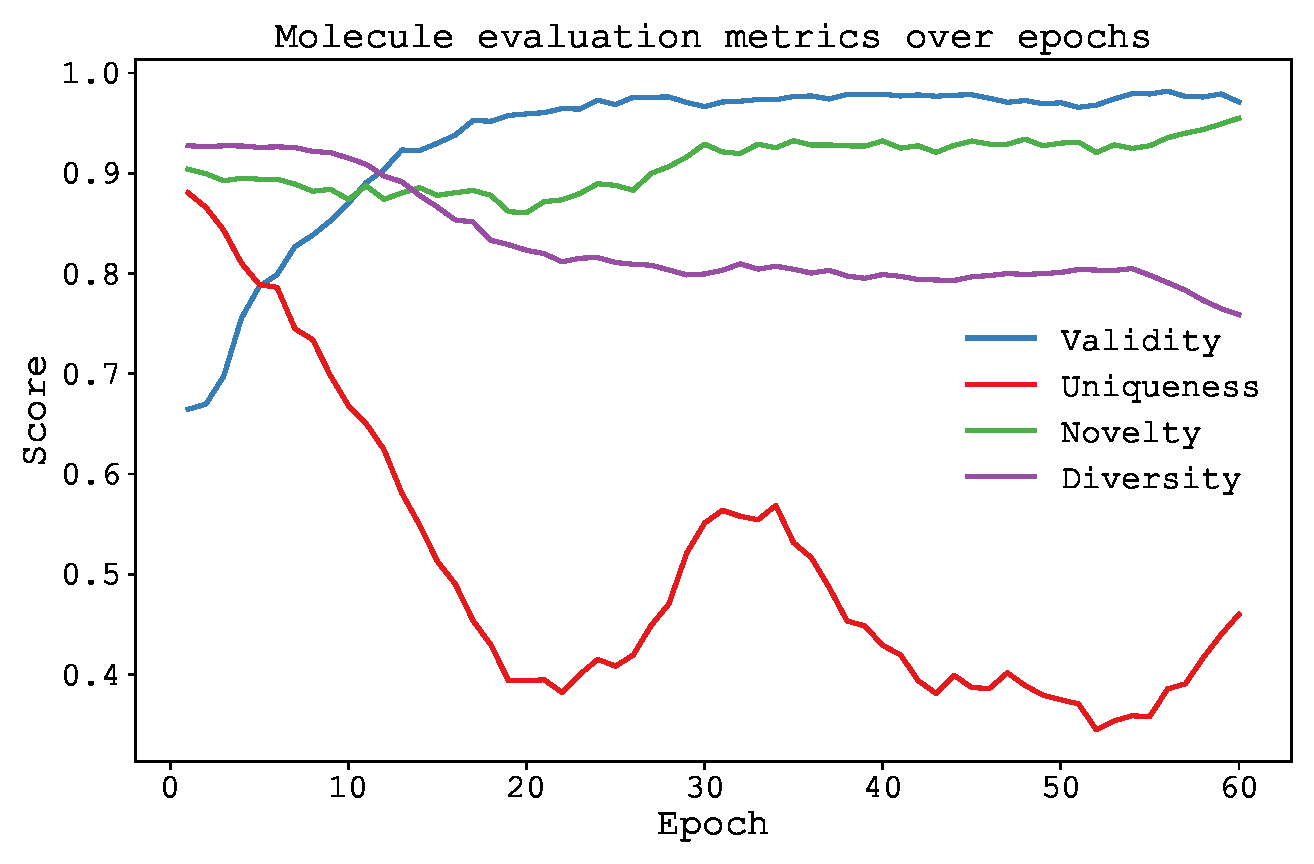
\includegraphics[width=0.8\textwidth]{figures/eval_metrics_epochs.pdf}
  \caption{Example of evolution of TenGAN metrics over epochs. }
  \label{fgr:example}
\end{figure}

\begin{figure}
  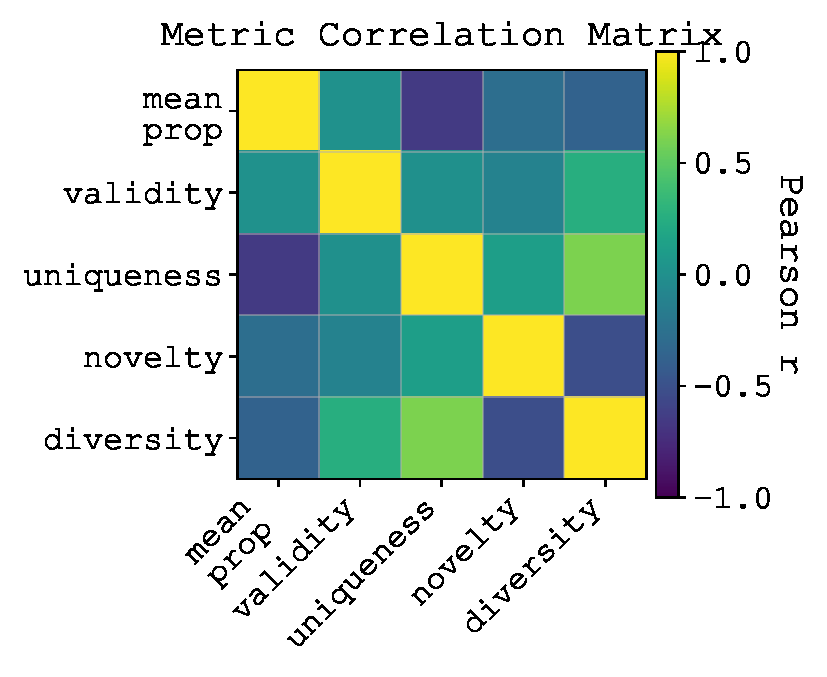
\includegraphics[width=0.5\textwidth]{figures/metric_corr.pdf}
  \caption{Heat map of performance metrics from hyperparameter optimisation. }
  \label{fgr:heatMap}
\end{figure}

\begin{figure}
  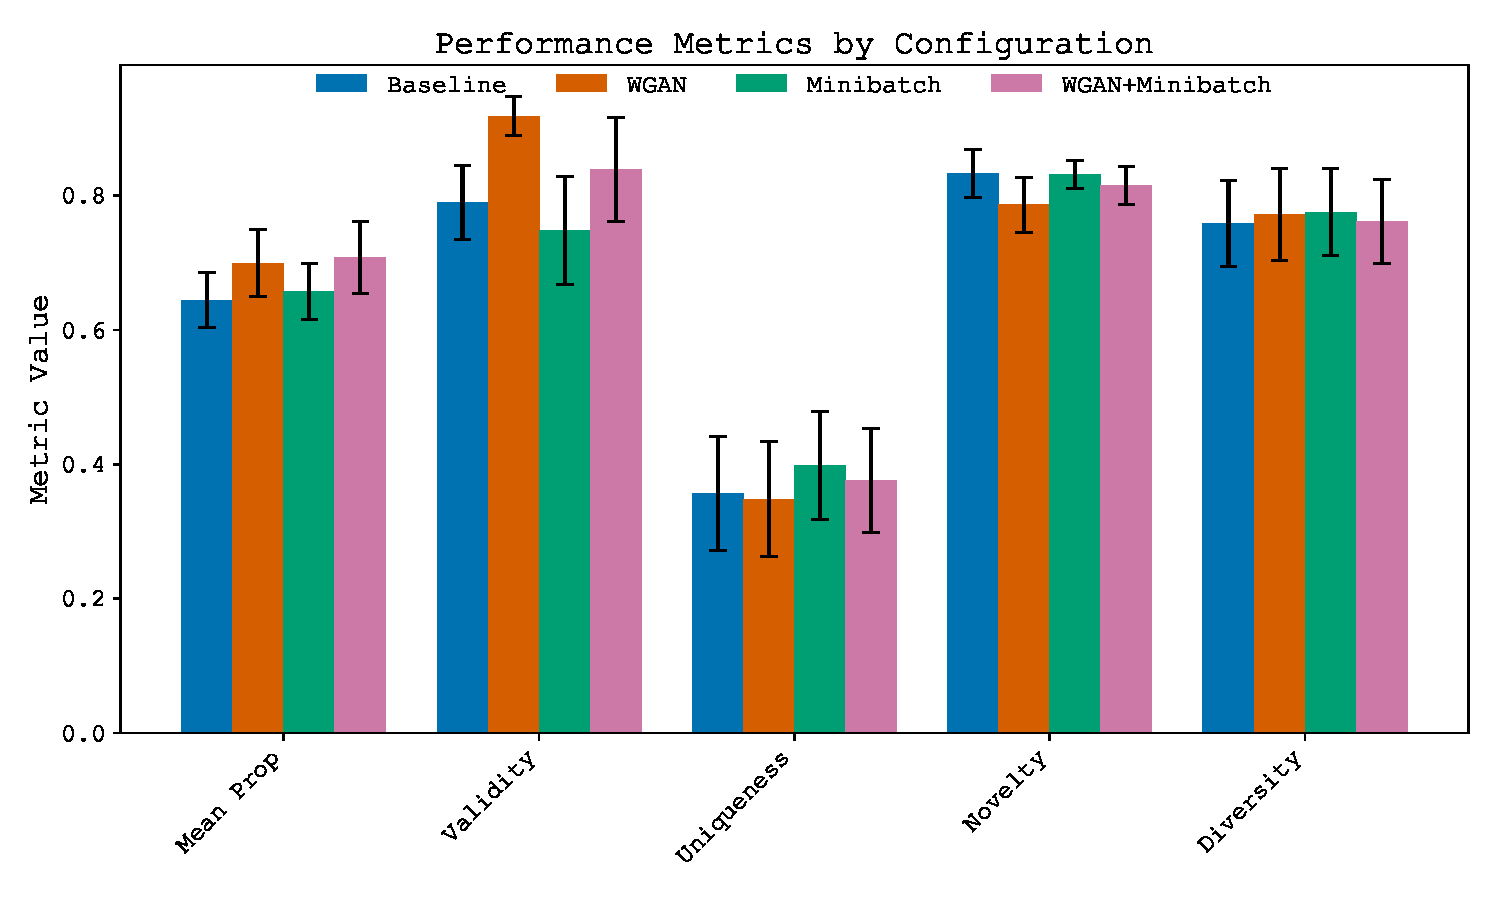
\includegraphics[width=1\textwidth]{figures/grouped_bar_metrics_colorblind.pdf}
  \caption{Effect of Wasserstein Distance and Mini-Batch discrimination on the output evaluation metrics. }
  \label{fgr:example}
\end{figure}


\section{Discussion}
internal and external. internal - compare model to itself; external - compare my results to what is SOTA. 

\section{Conclusion}
answer to the problem that we were trying to solve. open for perspectives. 

\section{Outline}

\subsection{Floats}

New float types are automatically set up by the class file.  The
means graphics are included as follows (Scheme~\ref{sch:example}).  As
illustrated, the float is ``here'' if possible.
\begin{scheme}
  Your scheme graphic would go here: \texttt{.eps} format\\
  for \LaTeX\, or \texttt{.pdf} (or \texttt{.png}) for pdf\LaTeX\\
  \textsc{ChemDraw} files are best saved as \texttt{.eps} files:\\
  these can be scaled without loss of quality, and can be\\
  converted to \texttt{.pdf} files easily using \texttt{eps2pdf}.\\
  %\includegraphics{graphic}
  \caption{An example scheme}
  \label{sch:example}
\end{scheme}

\begin{figure}
  As well as the standard float types \texttt{table}\\
  and \texttt{figure}, the class also recognises\\
  \texttt{scheme}, \texttt{chart} and \texttt{graph}.
  \caption{An example figure}
  \label{fgr:example}
\end{figure}

\subsection{Maths}
Some inline material \( y = mx + c \) or $ 1 + 1 = 2 $
followed by some display. \[ A = \pi r^2 \]

It is possible to label equations in the usual way (Eq.~\ref{eqn:example}).
\begin{equation}
  \frac{\mathrm{d}}{\mathrm{d}x} \, r^2 = 2r \label{eqn:example}
\end{equation}

\subsection{Tables}

\begin{table}
  \caption{An example table}
  \label{tbl:example}
  \begin{tabular}{ll}
    \hline
    Header one  & Header two  \\
    \hline
    Entry one   & Entry two   \\
    Entry three & Entry four  \\
    Entry five  & Entry five  \\
    Entry seven & Entry eight \\
    \hline
  \end{tabular}
\end{table}



%%%%%%%%%%%%%%%%%%%%%%%%%%%%%%%%%%%%%%%%%%%%%%%%%%%%%%%%%%%%%%%%%%%%%
%% The "Acknowledgement" section can be given in all manuscript
%% classes.  This should be given within the "acknowledgement"
%% environment, which will make the correct section or running title.
%%%%%%%%%%%%%%%%%%%%%%%%%%%%%%%%%%%%%%%%%%%%%%%%%%%%%%%%%%%%%%%%%%%%%
\begin{acknowledgement}
The author thanks Dr. Zied Hosni (Institute of Materials Discovery, University College London, UK) for supervision and guidance. The author acknowledges the use of the UCL Myriad High Performance Computing Facility (Myriad@UCL), and associated support services, in the completion of this work. 

\end{acknowledgement}

%%%%%%%%%%%%%%%%%%%%%%%%%%%%%%%%%%%%%%%%%%%%%%%%%%%%%%%%%%%%%%%%%%%%%
%% The same is true for Supporting Information, which should use the
%% suppinfo environment.
%%%%%%%%%%%%%%%%%%%%%%%%%%%%%%%%%%%%%%%%%%%%%%%%%%%%%%%%%%%%%%%%%%%%%
\begin{suppinfo}

Model files, GAN and Gaussian 16 log files, as well as scripts for figures available on: \\ \url{https://github.com/ZiedHosni1/ZH5_Karl}
\\ Should include all log files from gaussian, orbitals, python files, etcetc. Some will selectively go into the main text. 

\end{suppinfo}

%%%%%%%%%%%%%%%%%%%%%%%%%%%%%%%%%%%%%%%%%%%%%%%%%%%%%%%%%%%%%%%%%%%%%
%% The appropriate \bibliography command should be placed here.
%% Notice that the class file automatically sets \bibliographystyle
%% and also names the section correctly.
%%%%%%%%%%%%%%%%%%%%%%%%%%%%%%%%%%%%%%%%%%%%%%%%%%%%%%%%%%%%%%%%%%%%%
\bibliography{references}

\end{document}
